
%%%%%%%%%%%%%%%%%%%%%%%%%%%%%%%%%%%%%%%%%%%%%%%%%%%%%%%%%%%%%%%%%%%%%%%%%%%%%%%%
%%%%%%%%%%% Document class and package options
%%%%%%%%%%%%%%%%%%%%%%%%%%%%%%%%%%%%%%%%%%%%%%%%%%%%%%%%%%%%%%%%%%%%%%%%%%%%%%%%
% \documentclass[a4paper,12pt]{article}
\documentclass[a4paper,12pt,twoside]{article}
\usepackage{outline}

\usepackage{amsmath}
\usepackage{amssymb}                    % AMS Math
\usepackage{amsfonts}
\usepackage[tight,hang,centerlast]{subfigure}
\usepackage[lined,ruled,longend]{algorithm2e}
\usepackage{longtable}
\usepackage{verbatim}

%\usepackage[dvipsnames]{xcolor}

\usepackage{rotating}

\usepackage{fancyvrb}




\clubpenalty=1000
\widowpenalty=1000

%% eps to pdf
%% specify .eps extension when \includegraphics if you want the .pdf fig file to
%%     be regenerated as part of the compilation. Without extension the .pdf fig
%%     file is generated only if it does not exist yet
%% --shell-escape option must be enabled
\newif\ifpdf
\ifx\pdfoutput\undefined
   \pdffalse
\else
   \pdfoutput=1
   \pdftrue
\fi
\ifpdf
   \usepackage{graphicx}
   \usepackage{epstopdf}

   \epstopdfsetup{suffix=}

   \DeclareGraphicsRule{.eps}{pdf}{.pdf}{`epstopdf #1}
   \pdfcompresslevel=9
\else
   \usepackage{graphicx}
\fi

% redefine \VerbatimInput
\RecustomVerbatimCommand{\VerbatimInput}{VerbatimInput}%
{fontsize=\tiny,
 %
 frame=lines,  % top and bottom rule only
 framesep=2em, % separation between frame and text
% rulecolor=\color{Gray},
 %
 label=\fbox{ping.stat},
 labelposition=topline,
 %
 commandchars=\|\(\), % escape character and argument delimiters for
                      % commands within the verbatim
 commentchar=*        % comment character
}

\begin{document}


%%%%%%%%%%%%%%%%%%%%%%%%%%%%%%%%%%%%%%%%%%%%%%%%%%%%%%%%%%%%%%%%%%%%%%%%%%%%%%%%
%%%%%%%%%%% Title
%%%%%%%%%%%%%%%%%%%%%%%%%%%%%%%%%%%%%%%%%%%%%%%%%%%%%%%%%%%%%%%%%%%%%%%%%%%%%%%%

\title{Measurement Results from\\
Wireless Battle Mesh\\
Version 7}


%\date{Mai, 2014}

\contributors{WBM community}
\eventlocation{Sublab. Leipzig, Germany}
\eventdates{12th to 18th of May 2014}
\eventurl{http://battlemesh.org/BattleMeshV7}
\doctype{Measurement Analysis (work in progress)}
\logofigure{figures/battlemeshv7}

\frontmatter

\maketitle

%%%%%%%%%%%%%%%%%%%%%%%%%%%%%%%%%%%%%%%%%%%%%%%%%%%%%%%%%%%%%%%%%%%%%%%%%%%%%%%%
%%%%%%%%%%% Indices
%%%%%%%%%%%%%%%%%%%%%%%%%%%%%%%%%%%%%%%%%%%%%%%%%%%%%%%%%%%%%%%%%%%%%%%%%%%%%%%%

\thispagestyle{plain}
%\vspace*{3cm}

%\begin{center}
%\LARGE{\textbf{Abstract}} 
%\end{center}

%\begin{itemize}
%\item TODO..
%\end{itemize}

%\cleardoublepage
\clearsinglepage

\thispagestyle{plain}
\tableofcontents

%\cleardoublepage
\clearsinglepage

%%%%%%%%%%%%%%%%%%%%%%%%%%%%%%%%%%%%%%%%%%%%%%%%%%%%%%%%%%%%%%%%%%%%%%%%%%%%%%%%
%%%%%%%%%%% The document
%%%%%%%%%%%%%%%%%%%%%%%%%%%%%%%%%%%%%%%%%%%%%%%%%%%%%%%%%%%%%%%%%%%%%%%%%%%%%%%%

\singlespacing
\mainmatter
%%%%%%%%%%%%%%%%%%%%%%%%%%%%%%%%%%%%%%%%%%%%%%%%%%%%%%%%%%%%%%%%%%%%%%%%%%%%%%%%
%%%%%%%%%%% Chapter Inclusion
%%%%%%%%%%%%%%%%%%%%%%%%%%%%%%%%%%%%%%%%%%%%%%%%%%%%%%%%%%%%%%%%%%%%%%%%%%%%%%%%


%%%%%%%%%%%%%%%%%%%%%%%%%%%%%%%%%%%%%%%%%%%%%%%%%%%%%%%%%%%%%%%%%%%%%%%%%%%%%%%%
%%%%%%%%%%%%%%%%%%%%%%%%%%%%%%%%%%%%%%%%%%%%%%%%%%%%%%%%%%%%%%%%%%%%%%%%%%%%%%%%
\thispagestyle{plain}

%%%%%%%%%%%%%%%%%%%%%%%%%%%%%%%%%%%%%%%%%%%%%%%%%%%%%%%%%%%%%%%%%%%%%%%%%%%%%%%%
%%%%%%%%%%%%%%%%%%%%%%%%%%%%%%%%%%%%%%%%%%%%%%%%%%%%%%%%%%%%%%%%%%%%%%%%%%%%%%%%
%%%%%%%%%%%%%%%%%%%%%%%%%%%%%%%%%%%%%%%%%%%%%%%%%%%%%%%%%%%%%%%%%%%%%%%%%%%%%%%%
\section{Introduction}
\label{sec:introduction}


WBM...

%%%%%%%%%%%%%%%%%%%%%%%%%%%%%%%%%%%%%%%%%%%%%%%%%%%%%%%%%%%%%%%%%%%%%%%%%%%%%%%%
%%%%%%%%%%%%%%%%%%%%%%%%%%%%%%%%%%%%%%%%%%%%%%%%%%%%%%%%%%%%%%%%%%%%%%%%%%%%%%%%
%%%%%%%%%%%%%%%%%%%%%%%%%%%%%%%%%%%%%%%%%%%%%%%%%%%%%%%%%%%%%%%%%%%%%%%%%%%%%%%%
% A summary of protocol itself, the used versions and configuration

%\section{Protocols}


%\subsection{Babel}

%\subsection{Batman-adv}

%\subsection{Bmx6}

%\subsection{OLSR}

\section{Data and System Repositories}

\begin{rawtext}[caption={Testbed and experiment related code and data repositories}, label=resources]
http://wibed.confine-project.eu

https://github.com/battlemesh/wibed (buildroot)
https://github.com/battlemesh/wibed-battlemesh-experiment (package)
http://wiki.confine-project.eu/wibed:start
https://github.com/axn/wbm2pdf  (this stuff, branch wbmv7 in future)

Raw measurement data:
http://wibed.confine-project.eu/resultsdir/wbmv7-axn-16_2014-05-16_19-28-43 (stationary scenarios)
http://wibed.confine-project.eu/resultsdir/wbmv7-axn-17_2014-05-16_20-13-20 (broken crossed streams scenario)
http://wibed.confine-project.eu/resultsdir/wbmv7-axn-19_2014-05-16_21-35-33 (mobile scenarios)

\end{rawtext}


%%%%%%%%%%%%%%%%%%%%%%%%%%%%%%%%%%%%%%%%%%%%%%%%%%%%%%%%%%%%%%%%%%%%%%%%%%%%%%%%
%%%%%%%%%%%%%%%%%%%%%%%%%%%%%%%%%%%%%%%%%%%%%%%%%%%%%%%%%%%%%%%%%%%%%%%%%%%%%%%%
%%%%%%%%%%%%%%%%%%%%%%%%%%%%%%%%%%%%%%%%%%%%%%%%%%%%%%%%%%%%%%%%%%%%%%%%%%%%%%%%
\section{Testbed ad Experiment Descripiton}

\subsection{Deployment}

During the first days of the event a total of 20 wibed nodes have been
deployed. 16 wibed-nodes have beend spread over 3 different floors in
the main event building. About 10 of these 16 nodes were located in
the main event hall (approximately 300 sqare-meters workshop room)
with highest node density in a particular corner of this room
(deathroom in Note \ref{locations}) and the 6 in the below and above floor of the event
hall. Three more nodes have been placed in a neighboring building with
wireless connectivity.  One node was battery powerded for allowing
mobile-node scenarios.  In fact not all node positions were always
exactly known as nodes were sometimes moved to fullfill specific
experimentation-scenario requirements.  In each building 1 of the
wibed-nodes were configured as GW nodes and blocked for experimental
usage. The remaining 18 nodes were shared between three different
experimentation groups for running tests and different scenarios (each
node was used by at most one experimentation group at any time).

All experiments were performed in a single 5Ghz channel. However, due
to the presence of around 50 participans with wireless laptops and
several other actively used wireless equipment, also the used 5GHz
channel was likely affected by non-testbed related interference.

The experiment presented in this work was lead by one of these groups
and used the following 16 nodes:

\begin{rawtext}[caption={Node locations and experiment usage}, label=locations]
NodeID  Location               exp:axn-16   exp:axn-19
                               (stationary) (mobile)
164a7a  deathroom
3b3a90  workshopRoom
3b3d70  ????
3e9db0  deathroom??            9db0->1ab0  9db0->4174
51aac8  halleAnfang                        aac8->4174
8a417e  deathroom              417e->4174   
c24174  HalleEnde (mobile)                  
c2427a  deathroom??                        427a->4174
ce3360  EloiTable
e4b63a  mustiTable
e60a62  halleMitte
e60aac  deathroom
e60ad6  deathroom
e61936  axelsTable             1936->4174  1936->4174
f41ab0  kloschi (building B)   1ab0->4174  1ab0->4174
\end{rawtext}


\subsection{Protocol Configurations and Assumptions}
The highly dynamic and uncontrollable interference in the measurement
environment made it inpossible to ensure equal conditions for
sequential experiment executions. Therefore, to ensure equal (fair)
environment conditions for all tested protocols, all routing protocols
were running and observed in parallel on all nodes, thus all being
always exposed to the exactly same environmental conditions. 

The accepted downside of this approach is of course that protocol
overhead introduced by one protocol or by protocol-observing tools
like ping (causing total overhead in the order of few KB/s, as can be
seen from later measurements) slightly affects the maximum achievable
end-to-end throughput of other protocols (in the order of seveal
MB/s).

Only netperf-tcp-based throughput probes, seeking to measure the
achievable tcp performance of the end-to-end routing paths established
by the individual protocols, were performed sequentially. This
decision has been made because each netperf test trys to load the
capacity of a given end-to-end path with a maximum of traffic, thus
introducing maximum probing-traffic overhead and interference while on
the other hand (given the tcp-inherent exponential backoff approach)
drastically lowering the currently offered load in the presence of
packet loss, leading to highly randomized results when running in
parallel and making the comparatin of parallel executions difficult.


All protocols were configured for routing IPv6 traffic using an
individual ULA address prefix per protocol. 

All protocols were configured with default parametrizations, thus no
environment specific customizations have been made apart from ensuring
the routing of the given IPv6 address range. The exact configuration
can be accessed via \cite{wbm-config}.

To avoid protocol-bootstrapping effects (eg unfinished neighbor-,
path- or topology-discovery), all routing protocol deamons were
started at least 200 seconds before any measurement.

\subsection{Measurement Configuration and Assumptions}
\label{measurement-config}

Followup measurements were executed from a singe selected node
(src-node) by launching a pre-deployed test script \cite{wbm-test} and
given the id of a single other node (dst-node) for probing end-to-end
path characteristics. Src-node and dst-node IDs for each measurement
are given in Note \ref{locations}.

Each followup measurement last 200 seconds during which the following
additional tools were used to observe protocol performance and
overhead: 
\begin{itemize}
\item ping6 (unix) command to dst-node ipv6 address with one-second interval
  and 1000 bytes icmp user data. The output of the ping6 command got
  logged for later end-to-end packet loss, hop-count, and round-trip
  time (RTT) over time analysis.

\item top (unix) command for logging protocol-specific CPU and memory
  consumption at 1 second intervals.

\item mtr (my trace route, unix) command at 1 second interval for
  tracing full src-to-dst protocol-established path information. Due
  to the difficulty to correlate or graphically represent these traces,
  the obtained log files were not processed further.

\item netperf, executed in repeating rounds (4 rounds), each probing
  sequentially the maximum achievable end-to-end throughput to always
  the same destination node for 10 seconds via each routing protocol.
  
\item tcpdump, passively capturing the present routing-protocol
  overhead of each protocol as reveived on the wireless channel by the
  src node.

\end{itemize}

\subsection{Experiments}

The experiment focused on measuring the overhead and performance of 5
different mesh routing protocol implementations in static and mobile
scenarios. The five tested protocols were batman-advanced (batadv),
bmx6, olsr, olsr2, and babel. Unfortunately, we just discovered after
the measurements that the babel protocol daemon was not configured
correctly, leading to broken routing decisions for multi-hop
path. Therefore all babel-protocol related measurements were discareded
in the following discussion.

Experiments are grouped in two different scenarios (wibed experiments
with results accessible via corresponding wibed-data repositories as
given in Note \ref{resources} for exp-16 and exp-19 ), each scenario
consisted of about 4 measurement executions by using different
source-destination combinatinos (measurement results were stored on
the source-node of the measurement as given by Note \ref{locations}).
In the following the two scenarios and selected measrurement results
are discussed.  The complete set of obtained measurement results and
resulting graphs are given graph tables \ref{tbl:s-pings} to
\ref{tbl:m:4}.

\subsubsection{Stationary scenario}

During the stationary scenario the involved wibed nodes were not
moved, however still affected by uncontrollable interference
conditions from the environment itself, other parallel experiments
executed on other wibed nodes, and the traffic created by the
experiments itself. For each measurement a different couple of
source-node and destinatino-node was selected intuitively with the
objective to select, in terms of network-topology, rather distant
(so non-neighboring) nodes.

Each selected node couple was tested successively (with several
hundreds seconds between each measurement) over 200 seconds using the
wbm-test script \cite{wbm-test} doing measurements as described in
Section \ref{measurement-config}.

\subsubsection{Mobile scenario}

Apart from the presence of a single mobile node, always serving as
destination node, all mobile scenarios were performed in the same way
as the stationary scenarios. During the mobile scenario the mobile
node was moved (carried) manually at slow-walking speed (approximately
1m/second) the about 100 meters back and forth along the main event
hall, downstairs to the lower floor, and along the lower hall.  The
mobile-node carrying walker returned to its original position few
seconds before the end of each 200seconds lasting measurement.


\subsection{Discussion of Measurement Results}

In the following the results of only one performed measurement are
discussed in more detail. Therefore the last measurement, as summarized
via graphs in Table \ref{tbl:s4}, was selected simply beacause it
suited best to illustrate a number of expected and unexpected
phenomenas. The results represented by this selection are by no means
representive. However, looking at all perfromed measurements, a
general ranking of protocols can only be done regarding a very few
particular characteristics while for other, given the few number of
measurements and the high amount of randomness involved, at most some
vague tendencies may be guessed.

The protocol traffic overhead in terms of




% wget http://downloads.battlemesh.org/WBMv6/geographical_map1.png
% wget http://downloads.battlemesh.org/WBMv6/geographical_map2.png
%\begin{figure}[!ht]
%\centering
%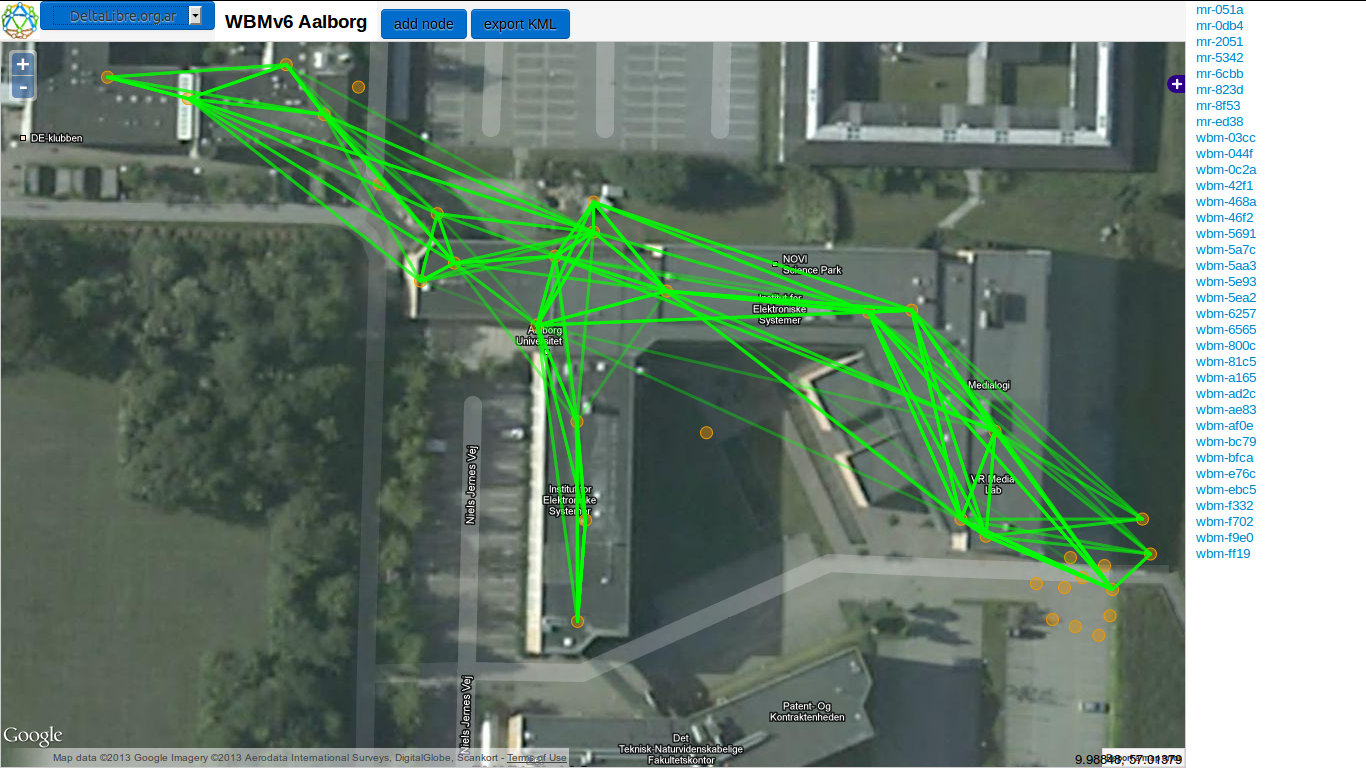
\includegraphics[width=1.4\textwidth, angle=90]{figures/geographical_map2.png}
%\caption{geographical map snapshot}
%\label{fig:geomap}
%\end{figure}


% wget -O topo0.svg "http://battlemesh.org/BattleMeshV6/Tests?action=AttachFile&do=get&target=topo0.svg"
% \immediate\write18{ inkscape -D -z --file=topo0.svg --export-pdf=topo0.pdf }

%\begin{figure}[!ht]
%\centering
%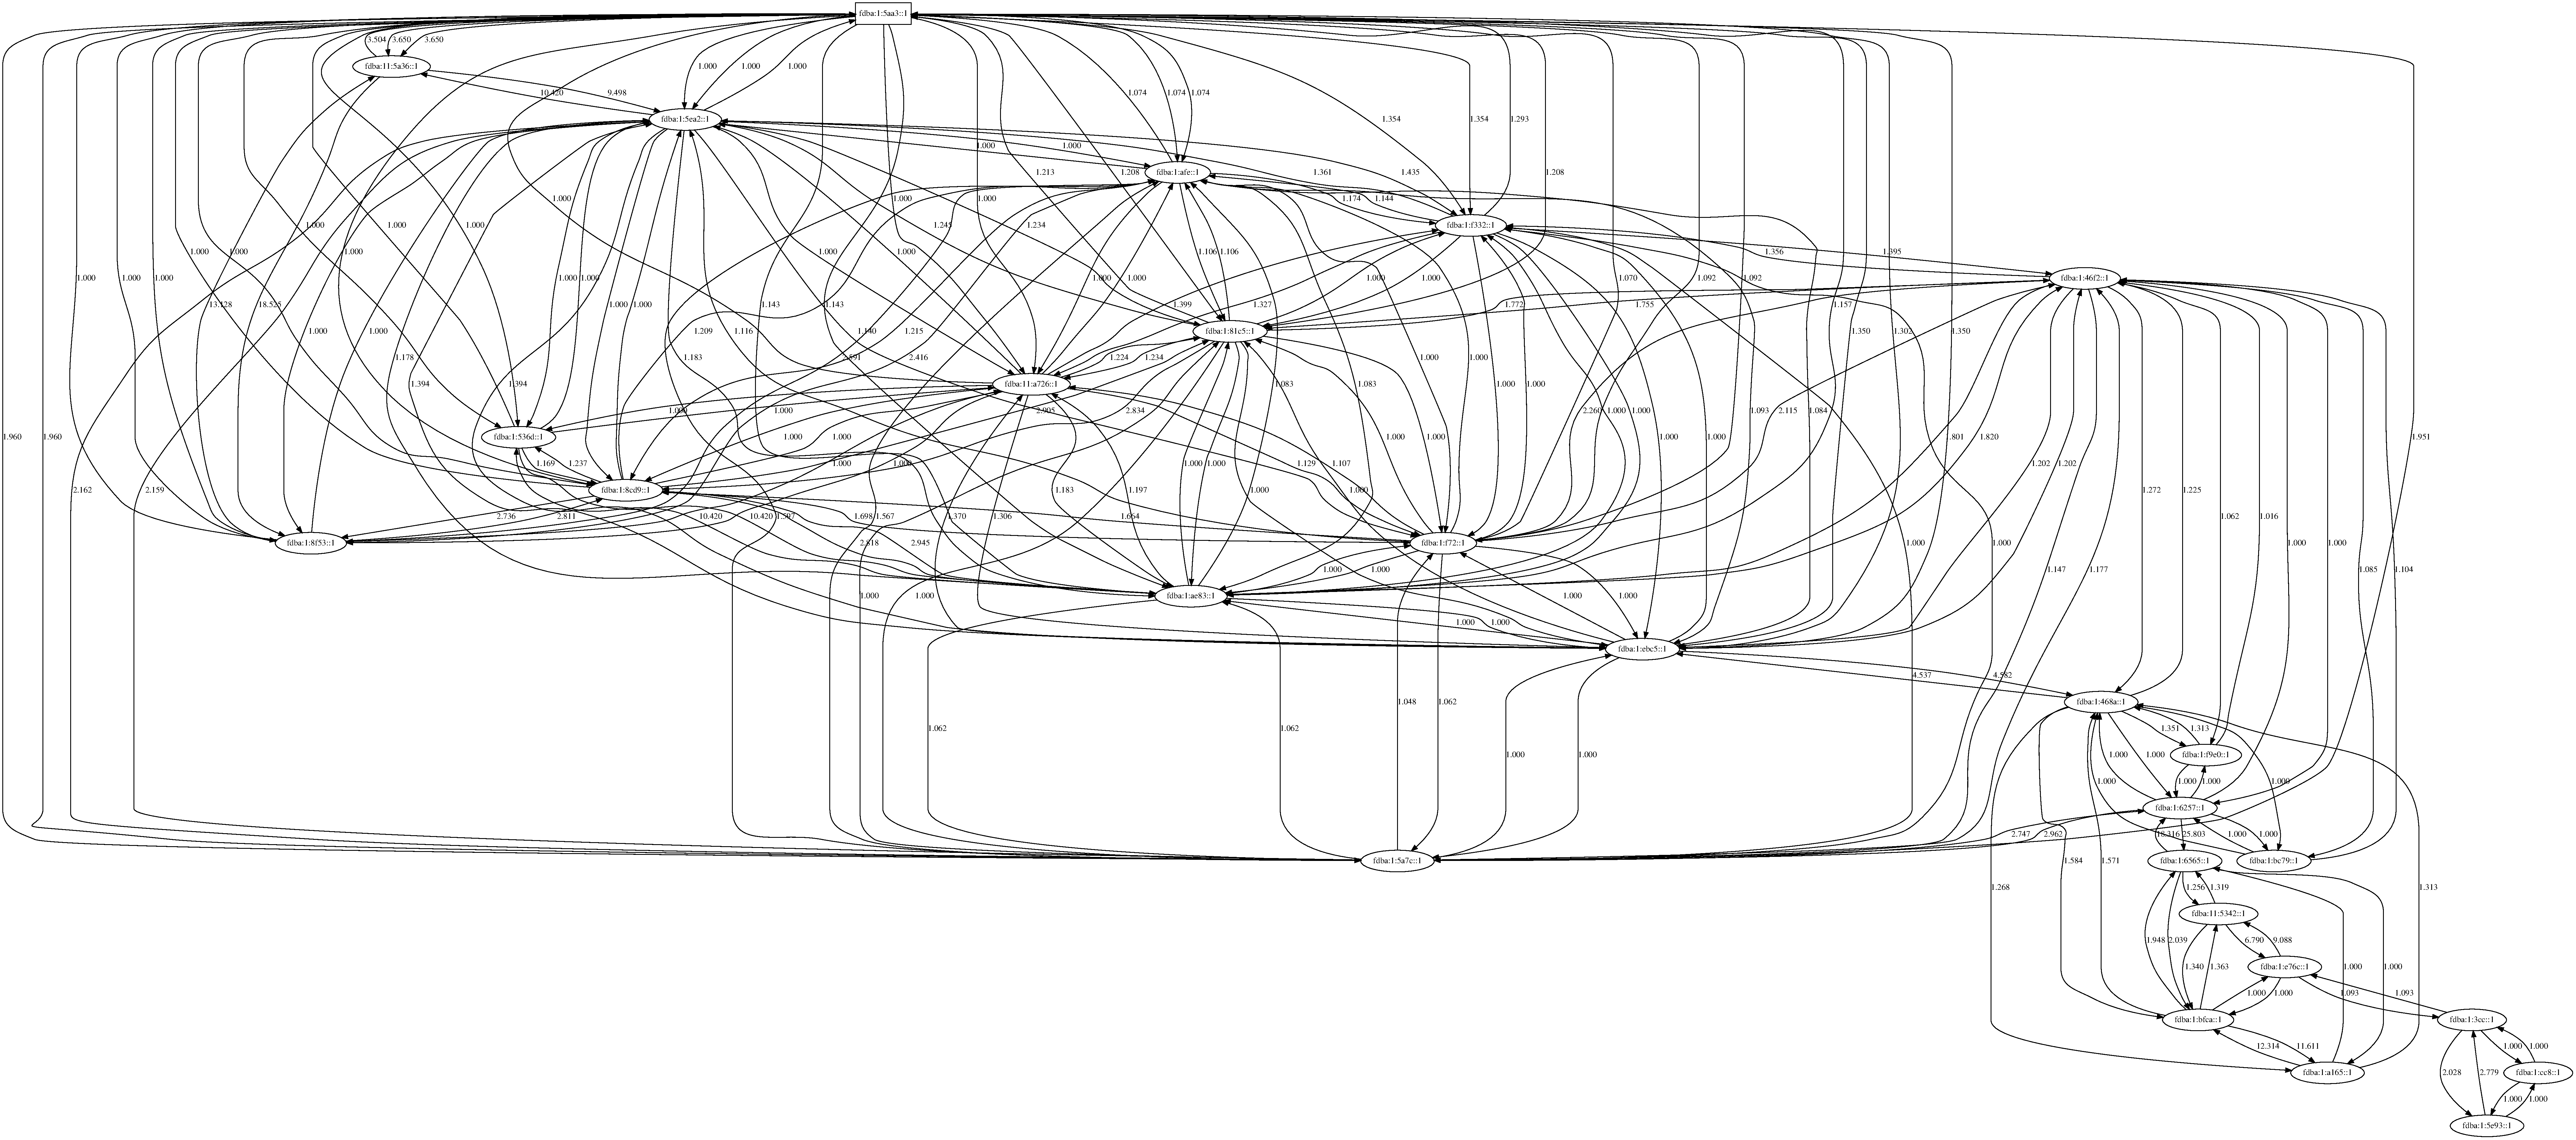
\includegraphics[width=1.4\textwidth, angle=90]{figures/topo0.pdf}
%\caption{OLSR topology snapshot}
%\label{fig:olsr-topo}
%\end{figure}

%\begin{figure}[h]
%\centering
%\def\svgwidth{\columnwidth}
%\includesvg{topo0}
%\end{figure}

\clearpage
%\makeFigure{sBrtt}{Random node test 2}{0.69}
%\makeFigure{sBrvh}{Random node test 2}{0.69}
%\immediate\write18{ ../eval.R --data=../tmp.data --stat=../tmp.stat --imgdir=../img --texdir=inputs/ }


\subsection{Stationary Nodes Measurements}

\makeCCCTabl{tbl:s-pings}{End-to-end ping6 performance between two stationary nodes: 9db0-1ab0, 417e-4174, 1936-4174, 1ab0-4174} {%
%  \makeCCCPingGraphic{}
  \makeCCCPingGraphic{./test_data/wbmv7-axn-16_2014-05-16_19-28-43/wbmv7-axn-16_2014-05-16_19-28-43_wibed-3e9db0/wbm-axn}
  \makeCCCPingGraphic{./test_data/wbmv7-axn-16_2014-05-16_19-28-43/wbmv7-axn-16_2014-05-16_19-28-43_wibed-8a417e/wbm-axn}
  \makeCCCPingGraphic{./test_data/wbmv7-axn-16_2014-05-16_19-28-43/wbmv7-axn-16_2014-05-16_19-28-43_wibed-e61936/wbm-axn}
  \makeCCCPingGraphic{./test_data/wbmv7-axn-16_2014-05-16_19-28-43/wbmv7-axn-16_2014-05-16_19-28-43_wibed-f41ab0/wbm-axn}
}



\makeCCCTabl{tbl:s1}{Overhead and end-to-end performance between two stationary nodes: 3e9db0 and 1ab0} {%
  \makeCCCPingGraphic{./test_data/wbmv7-axn-16_2014-05-16_19-28-43/wbmv7-axn-16_2014-05-16_19-28-43_wibed-3e9db0/wbm-axn}
  \makeCCCPerfGraphic{./test_data/wbmv7-axn-16_2014-05-16_19-28-43/wbmv7-axn-16_2014-05-16_19-28-43_wibed-3e9db0/wbm-axn}
  \makeCCCOvhdGraphic{./test_data/wbmv7-axn-16_2014-05-16_19-28-43/wbmv7-axn-16_2014-05-16_19-28-43_wibed-3e9db0/wbm-axn}
}

\makeCCCTabl{tbl:s2}{Overhead and end-to-end performance between two stationary nodes: 8e417e and c24174} {%
  \makeCCCPingGraphic{./test_data/wbmv7-axn-16_2014-05-16_19-28-43/wbmv7-axn-16_2014-05-16_19-28-43_wibed-8a417e/wbm-axn}
  \makeCCCPerfGraphic{./test_data/wbmv7-axn-16_2014-05-16_19-28-43/wbmv7-axn-16_2014-05-16_19-28-43_wibed-8a417e/wbm-axn}
  \makeCCCOvhdGraphic{./test_data/wbmv7-axn-16_2014-05-16_19-28-43/wbmv7-axn-16_2014-05-16_19-28-43_wibed-8a417e/wbm-axn}
}

\makeCCCTabl{tbl:s3}{Overhead and end-to-end performance between two stationary nodes: e61936 and c24174} {%
  \makeCCCPingGraphic{./test_data/wbmv7-axn-16_2014-05-16_19-28-43/wbmv7-axn-16_2014-05-16_19-28-43_wibed-e61936/wbm-axn}
  \makeCCCPerfGraphic{./test_data/wbmv7-axn-16_2014-05-16_19-28-43/wbmv7-axn-16_2014-05-16_19-28-43_wibed-e61936/wbm-axn}
  \makeCCCOvhdGraphic{./test_data/wbmv7-axn-16_2014-05-16_19-28-43/wbmv7-axn-16_2014-05-16_19-28-43_wibed-e61936/wbm-axn}
}

\makeCCCTabl{tbl:s4}{Overhead and end-to-end performance between two stationary nodes: f41ab0 and c24174} {%
  \makeCCCPingGraphic{./test_data/wbmv7-axn-16_2014-05-16_19-28-43/wbmv7-axn-16_2014-05-16_19-28-43_wibed-f41ab0/wbm-axn}
  \makeCCCPerfGraphic{./test_data/wbmv7-axn-16_2014-05-16_19-28-43/wbmv7-axn-16_2014-05-16_19-28-43_wibed-f41ab0/wbm-axn}
  \makeCCCOvhdGraphic{./test_data/wbmv7-axn-16_2014-05-16_19-28-43/wbmv7-axn-16_2014-05-16_19-28-43_wibed-f41ab0/wbm-axn}
}


%\makeCCCTabl{tbl:p2}{concurrent End-to-end ping6 performance between four stationary nodes 1936-4174 and 1ab0-417e} {%
%  \makeCCCPingGraphic{./test_data/wbmv7-axn-17_2014-05-16_20-13-20/wbmv7-axn-17_2014-05-16_20-13-20_wibed-e61936/wbm-axn}
%  \makeCCCPingGraphic{./test_data/wbmv7-axn-17_2014-05-16_20-13-20/wbmv7-axn-17_2014-05-16_20-13-20_wibed-f41ab0/wbm-axn}
%}

%\makeCCCTabl{tbl:p3}{concurrent End-to-end ping6 performance between four stationary nodes 417e-1ab0 and 4174-1926} {%
%  \makeCCCPingGraphic{./test_data/wbmv7-axn-17_2014-05-16_20-13-20/wbmv7-axn-17_2014-05-16_20-13-20_wibed-8a417e/wbm-axn} %broken daemons
%  \makeCCCPingGraphic{./test_data/wbmv7-axn-17_2014-05-16_20-13-20/wbmv7-axn-17_2014-05-16_20-13-20_wibed-c24174/wbm-axn} %broken daemons
%}

\subsection{Mobile Node Measurements}

\makeCCCTabl{tbl:m-pings}{End-to-end ping6 performance to mobile node 4174 from aac8, 1936, 1ab0} {%
  \makeCCCPingGraphic{./test_data/wbmv7-axn-19_2014-05-16_21-35-33/wbmv7-axn-19_2014-05-16_21-35-33_wibed-51aac8/wbm-axn}
  \makeCCCPingGraphic{./test_data/wbmv7-axn-19_2014-05-16_21-35-33/wbmv7-axn-19_2014-05-16_21-35-33_wibed-e61936/wbm-axn}
  \makeCCCPingGraphic{./test_data/wbmv7-axn-19_2014-05-16_21-35-33/wbmv7-axn-19_2014-05-16_21-35-33_wibed-f41ab0/wbm-axn}
  \makeCCCPingGraphic{./test_data/wbmv7-axn-19_2014-05-16_21-35-33/wbmv7-axn-19_2014-05-16_21-35-33_wibed-c2427a/wbm-axn}
}


\makeCCCTabl{tbl:m1}{Overhead and end-to-end performance to mobile node c24174 from stationary node 51aac8} {%
  \makeCCCPingGraphic{./test_data/wbmv7-axn-19_2014-05-16_21-35-33/wbmv7-axn-19_2014-05-16_21-35-33_wibed-51aac8/wbm-axn}
  \makeCCCOvhdGraphic{./test_data/wbmv7-axn-19_2014-05-16_21-35-33/wbmv7-axn-19_2014-05-16_21-35-33_wibed-51aac8/wbm-axn}
}

\makeCCCTabl{tbl:m2}{Overhead and end-to-end performance to mobile node c24174 from stationary node e61936} {%
  \makeCCCPingGraphic{./test_data/wbmv7-axn-19_2014-05-16_21-35-33/wbmv7-axn-19_2014-05-16_21-35-33_wibed-e61936/wbm-axn}
  \makeCCCOvhdGraphic{./test_data/wbmv7-axn-19_2014-05-16_21-35-33/wbmv7-axn-19_2014-05-16_21-35-33_wibed-e61936/wbm-axn}
}

\makeCCCTabl{tbl:m3}{Overhead and end-to-end performance to mobile node c24174 from stationary node f41ab0} {%
  \makeCCCPingGraphic{./test_data/wbmv7-axn-19_2014-05-16_21-35-33/wbmv7-axn-19_2014-05-16_21-35-33_wibed-f41ab0/wbm-axn}
  \makeCCCOvhdGraphic{./test_data/wbmv7-axn-19_2014-05-16_21-35-33/wbmv7-axn-19_2014-05-16_21-35-33_wibed-f41ab0/wbm-axn}
}

\makeCCCTabl{tbl:m4}{Overhead and end-to-end performance to mobile node c24174 from stationary node c2427a} {%
  \makeCCCPingGraphic{./test_data/wbmv7-axn-19_2014-05-16_21-35-33/wbmv7-axn-19_2014-05-16_21-35-33_wibed-c2427a/wbm-axn}
  \makeCCCOvhdGraphic{./test_data/wbmv7-axn-19_2014-05-16_21-35-33/wbmv7-axn-19_2014-05-16_21-35-33_wibed-c2427a/wbm-axn}
}
%%%%%%%%%%%%%%%%%%%%%%%%%%%%%%%%%%%%%%%%%%%%%%%%%%%%%%%%%%%%%%%%%%%%%%%%%%%%%%%%
\subsection{Mobile Scenarios}



%\makeCCTabl{tbl:m0}{Mobile test 0 (group 1)} {%
%      \makeTCCGraphic{m0}
%}

%\makeCCTabl{tbl:m1}{Mobile node test 1 (group 2)} {%
%      \makeTCCGraphic{m1}
%}

%\makeCCTabl{tbl:m0-m2}{Running node test 2 (group 3)} {%
%      \makeTCCGraphic{m2}
%}




%%%%%%%%%%%%%%%%%%%%%%%%%%%%%%%%%%%%%%%%%%%%%%%%%%%%%%%%%%%%%%%%%%%%%%%%%%%%%%%%
%%%%%%%%%%%%%%%%%%%%%%%%%%%%%%%%%%%%%%%%%%%%%%%%%%%%%%%%%%%%%%%%%%%%%%%%%%%%%%%%
%%%%%%%%%%%%%%%%%%%%%%%%%%%%%%%%%%%%%%%%%%%%%%%%%%%%%%%%%%%%%%%%%%%%%%%%%%%%%%%%
\section{TCP Throughput Measurements}
\label{sec:tp-measurements}




\section{Recommendations for next battlemesh}

\begin{itemize}

\item Traceroute and mrt often show  high packet for intermediate nodes. This is due to a kind of denial-of-service mechanism enabled by default in Linux kernel. WIth this mechanism the kernel simply discards frequent icmp responses (eg due to exceeded TTL values). This behavior can be disabled by lowering the default net.ipv6.icmp.ratelimit=1000 setting, eg via: sysctl -w net.ipv6.icmp.ratelimit=10

\end{itemize}


%%%%%%%%%%%%%%%%%%%%%%%%%%%%%%%%%%%%%%%%%%%%%%%%%%%%%%%%%%%%%%%%%%%%%%%%%%%%%%%%
%%%%%%%%%%%%%%%%%%%%%%%%%%%%%%%%%%%%%%%%%%%%%%%%%%%%%%%%%%%%%%%%%%%%%%%%%%%%%%%%
%%%%%%%%%%%%%%%%%%%%%%%%%%%%%%%%%%%%%%%%%%%%%%%%%%%%%%%%%%%%%%%%%%%%%%%%%%%%%%%%
\section{Appendix}




%%%%%%%%%%%%%%%%%%%%%%%%%%%%%%%%%%%%%%%%%%%%%%%%%%%%%%%%%%%%%%%%%%%%%%%%%%%%%%%%
%%%%%%%%%%%%%%%%%%%%%%%%%%%%%%%%%%%%%%%%%%%%%%%%%%%%%%%%%%%%%%%%%%%%%%%%%%%%%%%%
%\section*{Acknowledgements}
%
%This work is supported by ...


%%%%%%%%%%%%%%%%%%%%%%%%%%%%%%%%%%%%%%%%%%%%%%%%%%%%%%%%%%%%%%%%%%%%%%%%%%%%%%%%
%%%%%%%%%%%%%%%%%%%%%%%%%%%%%%%%%%%%%%%%%%%%%%%%%%%%%%%%%%%%%%%%%%%%%%%%%%%%%%%%

\backmatter

\bibliographystyle{ieeetr}
%\bibliography{biblio-data}

\end{document} 
